\chapter{Data Understanding}

La fase che verrà descritta in seguito è fra le più delicate di tutto il processo di \textit{data mining}. Da essa dipende la buona riuscita o meno dell'intera attività di estrazione d'informazioni. Come appare quindi naturale, è stata dedicata a essa una particolare attenzione.

\section{Introduzione al Data Understanding}

\subsection{Scopo dell'Attività}

Perché occorre spendere del tempo per perpetrare un'estesa fase di \textit{data understanding}? \\

Banalmente, l'obiettivo principale che ci si prefigge è quello di ottenere una chiara visione di insieme sui dati che si hanno a disposizione. In questo modo, si sarà in grado di prendere decisioni oculate per quanto riguarda il da farsi nei successivi passi di questa analisi. Si prenda ad esempio l'attività di \textit{preprocessing}: sintetizzando al massimo, possiamo dire che si tratta di lavorare dei dati grezzi al fine di renderli a essere processati da certi algoritmi. L'ovvia implicazione è che occorre avere ben chiaro in anticipo quali algoritmi sarà opportuno lanciare, fatto che a sua volta implica la necessità di conoscere quali informazioni si intende estrarre dai dati grezzi a disposizione. \\

Questo aspetto rende necessario far precedere a quello che è, usando una metafora nell'ambito meccanico, l'attività di sgrossatura dei dati grezzi una fase di \textit{data understanding}. \\

In questa sezione, quindi, si punterà a capire a fondo la natura dei dati al fine d'intuire che cosa sia possibile trarne.

\subsection{Metodi e Strumenti}

L'attività di \textit{data understanding} può essere svolta in molti modi, non essendoci delle regole fisse che la disciplinano rigidamente. Si può azzardare che le risorse più importanti alle quali si può attingere in questo ambito sono, piuttosto romanticamente, l'intuito e la fantasia dei \textit{data scientist} coinvolti nel progetto. Fuori di metafora, è chiaro che non esistano procedure che indichino univocamente le informazioni che è possibile ricavare su un dato insieme di dati. Perciò, quello che occorre fare è sfruttare dei metodi che riassumano i dati per poterli apprezzare nel loro insieme. \\

Gli strumenti più adatti per poter ottenere una visione d'insieme sull'intera mole di dati sono, senza ombra di dubbio, le varie \textit{tecniche di visualizzazione} esistenti. Il loro utilizzo è stato permesso da software quali \textbf{R} e \textbf{Weka}, oltre che da più comuni \textit{spreadsheet} forniti da suite di programmi da ufficio. \footnote{Per un maggior dettaglio, si consulti il capitolo riguardo alla \textit{technology stack} impiegata per la realizzazione di questo progetto.}


\section{Dataset: Produttività degli Studenti}

\lstset{language=R,
    basicstyle=\small\ttfamily,
    stringstyle=\color{yellow},
    otherkeywords={0,1,2,3,4,5,6,7,8,9},
    morekeywords={TRUE,FALSE},
    deletekeywords={data,frame,length,as,character},
    keywordstyle=\color{blue},
    commentstyle=\color{green},
}

Senza ombra di dubbio questa porzione di dati rappresenta la più significativa dell'intero lotto a disposizione per questa analisi. \\

Si è quindi optato per utilizzare il software \textbf{R}, in quanto consente d'impiegare efficientemente un gran numero di approfondite tecniche di visualizzazione. Tuttavia, la potenza e la flessibilità offerte da questo tipo di strumento si pagano con la necessita di dedicare un minimo di attenzione all'importazione del dataset in quell'ambiente di lavoro. \\

In senso pratico, questo si traduce nel lanciare del codice analogo \footnotesize{--- non identico: sono stati accorciati i percorsi ---}\normalsize\ a quanto mostrato di seguito prima di poter effettuare qualunque altra operazione.

\newpage

\begin{lstlisting}
# set the repo root path before importing data!!!
setwd("C:/a/path/to/somewhere")
students <- read.csv("raw/prod_stud.csv")

# gather some info about the imported dataset
str(students)

# ADJUST DATA ATTRIBUTES 
# convert "coorte" to nominal by making it a factor 
students[, c(1)] <- sapply(students[, c(1)], factor)

# ok, let's take a look at it now
str(students)
summary(students)
\end{lstlisting}

In ogni caso, dato l’elevato numero degli attributi del dataset, è stato necessario fare delle scelte relative a cosa visualizzare – e con quale tecnica. Le scelte sono state ovviamente compiute su base intuitiva, a seguito di un’analisi sommaria delle caratteristiche del dataset. \\

È stato quindi deciso di effettuare una ricerca visiva di correlazioni fra valori di attributi relativi a:
\begin{itemize}
    \item prestazioni generali durante tutto il periodo esaminato
    \item prestazioni nei singoli esami
    \item risultati di gruppi di esami
\end{itemize}

\subsection{Prestazioni Generali degli Studenti}

Lo script \textbf{R} che segue plotta dei grafci di dispersione su coppie di attributi relativi alle prestazioni generali degli studenti. \\

\begin{lstlisting}
colors <- c("blue","red", "green", "orange")
coorte_labels <- students[,1]
coorte_colors <- colors[as.numeric(coorte_labels)]
library(seriation)


# general attributes
students_subset1 <- students[,-c(1, 6 : 45)]
pairs(students_subset1, col = coorte_colors,lower.panel = 	NULL,cex.labelsiris=2, pch=19, cex = 1.2)
par(xpd = TRUE)
legend(x = 0.05, y = 0.4, cex = 1,legend = 	as.character(levels(coorte_labels)),fill = unique(coorte_colors))
par(xpd = NA)
\end{lstlisting}

Lo scopo è quello di individuare visivamente delle correlazioni significative fra questi attributi. Come si può infatti vedere sul grafico generato dallo script, esistono varie correlazioni fra gli attributi considerati. Nel merito, la correlazione fra le quantità \textit{crediti totali} e \textit{crediti con voto} è tanto palese quanto banale: il primo ammontare contiene il secondo, e la loro differenza è minima. 

\begin{center}
	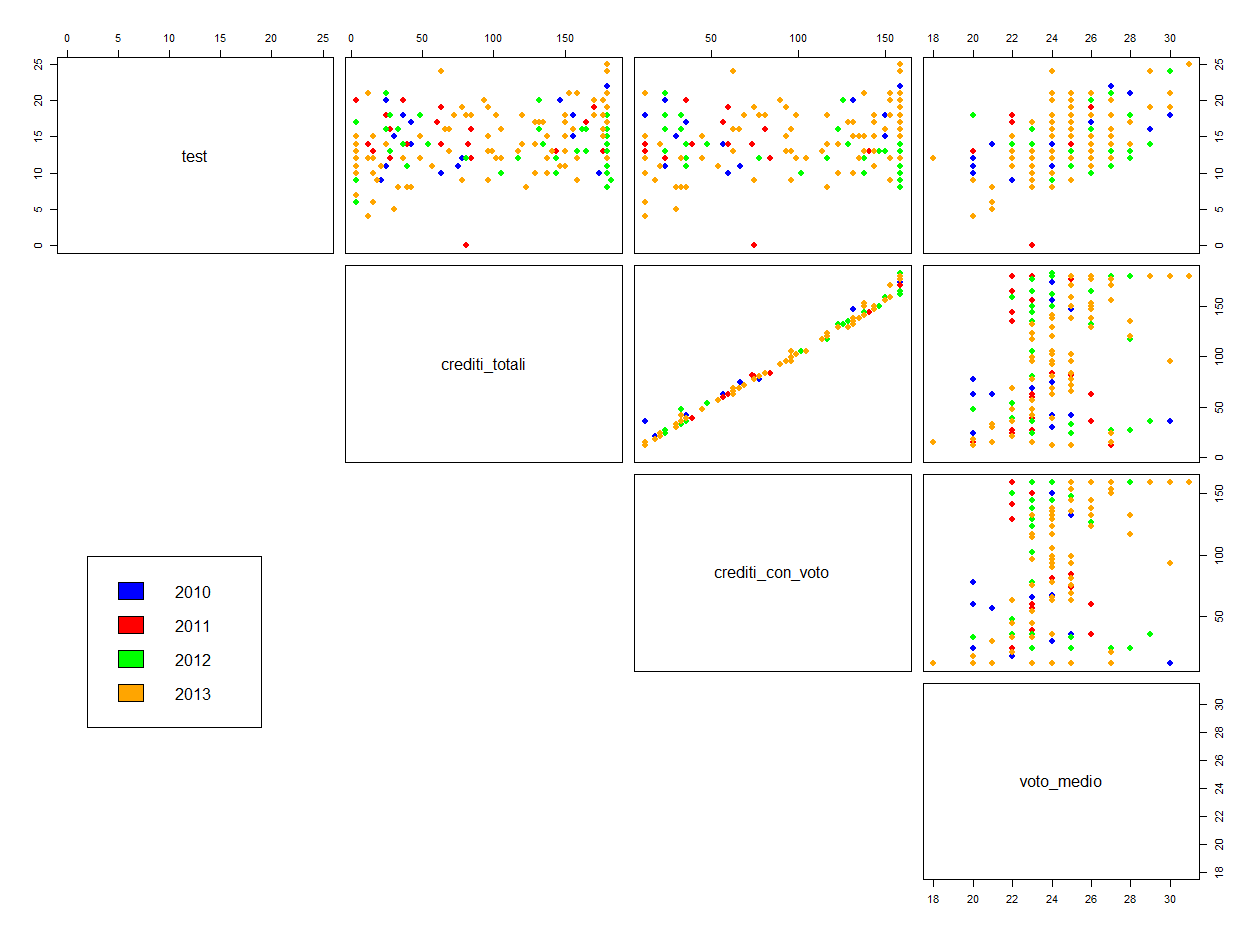
\includegraphics[scale=0.32]{img/scatter_plot_1_gen.png}
\end{center}